% !TeX root = ../main.tex

\chapter{相关理论和技术介绍}

在本章中,我们回顾一下实现编译器所需的基本工具。
程序通常由程序员以文本形式输入,即字符序列。程序作为文本的表示称为具体语法。
我们用具体语法简明地写下和讨论程序的语法。
在编译器中,我们使用抽象语法树来表示程序,因为编译器可以很方便高效地操作抽象语法树。
翻译具体语法到抽象语法的过程称作解析。
本文不涉及解析的理论和实现,一方面是因为现阶段解析已经有了相对固定化的套路和工具,研究也已经趋于完善。
另一方面由于本文选择了 Racket 作为源语言和实现语言,我们可以很方便地从字符串序列中构造出结构体,
而 Racket 的结构体也是本文选择的用以表示抽象语法树的数据结构。

\section{抽象语法树}

在计算机科学中,抽象语法树,或简称语法树,是源代码语法结构的一种抽象表示。
它以树状的形式表现编程语言的语法结构,树上的每个节点都表示源代码中的一种结构。
之所以说语法是“抽象”的,是因为这里的语法并不会表示出真实语法中出现的每个细节。
比如,嵌套括号被隐含在树的结构中,并没有以节点的形式呈现;
而类似于 if-condition-then 这样的条件跳转语句,可以使用带有三个分支的节点来表示。

\section{文法}

编程语言可以被看作是合法程序的集合,这一集合通常是无限大的,因为我们总是可以写出更加庞大复杂的程序。
因此,我们无法简单地通过把所有的合法程序列出来来描述一门语言。
通常,我们使用文法——一系列规则,来构造程序。文法通常用来描述具体语法,但它也可以被用来描述抽象语法。
本文使用巴科斯-诺尔范式\cite{Knuth_1964, Backus_Bauer_1960}的变体来描述我们的语言。
图\ref{fig:con-syntax-eg}中的几条规则给出了本文实现的语言的一个子集的描述,
该语言仅支持包含加减法的整数运算,但它允许任意复杂的嵌套表达式。

\begin{figure}[t]
  \fbox{
    \begin{minipage}{0.96\textwidth}
      \[
      \begin{array}{rcl}
        \Type & ::= & \key{Integer} \\
        \Exp & ::= & \Int \MID \LP\key{read}\RP \MID \LP\key{-}\;\Exp\RP \MID \LP\key{+} \; \Exp\;\Exp\RP \\
        \Lang & ::= & \Exp
      \end{array}
      \]
    \end{minipage}
  }
  \caption{具体语法示例}
  \label{fig:con-syntax-eg}
\end{figure}

\begin{figure}[t]
  \fbox{
    \begin{minipage}{0.96\textwidth}
      \[
      \begin{array}{rcl}
        \Type & ::= & \key{Integer} \\
        \Exp &::=& \INT{\Int} \MID \READ{} \MID \NEG{\Exp} \\
        &\MID&  \ADD{\Exp}{\Exp}  \\
        \LangInt{}  &::=& \PROGRAM{\code{'()}}{\Exp}
      \end{array}
      \]
    \end{minipage}
  }
  \caption{抽象语法示例}
  \label{fig:abs-syntax-eg}
\end{figure}

其中 \code{read} 函数读取用户在键盘上输入的一串数字,返回一个整数。
下面这行代码是这个示例语言一个完整的合法的程序:

\begin{lstlisting}
(+ (read) (- 8))
\end{lstlisting}

该程序对应的语法树如图\ref{fig:ast-eg}。

\begin{figure}[t]
  \begin{center}
      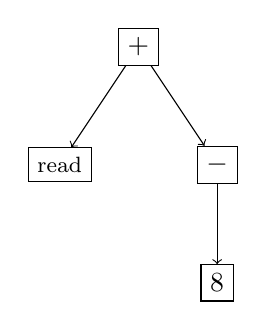
\begin{tikzpicture}
        \node[draw] (plus)  at (0 ,  0) {\key{+}};
        \node[draw] (read)  at (-1, -1.5) {{\footnotesize\key{read}}};

        \node[draw] (minus) at (1 , -1.5) {$\key{-}$};
        \node[draw] (8)     at (1 , -3) {\key{8}};

        \draw[->] (plus) to (read);
        \draw[->] (plus) to (minus);
        \draw[->] (minus) to (8);
      \end{tikzpicture}
  \end{center}
  \caption{语法树示例}
  \label{fig:ast-eg}
\end{figure}

\section{Racket 结构体和模式匹配}

图\ref{fig:con-syntax-eg}对应的抽象语法的描述如图\ref{fig:abs-syntax-eg}所示。
其中\code{Int},\code{Prim}等即为对应的Racket结构体的构造函数。
这些结构体可以非常简单地被定义出来:
\begin{lstlisting}
(struct Int (value))
(struct Prim (op args))
\end{lstlisting}

构造结构体也非常简单,下面这行代码对应的即为具体语法为\code{(+ (read) (- 8))}的程序:
\begin{lstlisting}
(Prim '+
      (list (Prim 'read '())
            (Prim '- (list (Int 8))))
\end{lstlisting}

而对结构体使用模式匹配,我们可以很方便地判断结构体的类型以及访问结构体的成员,以及语法树的子树。
例如,对于下面这段代码
\begin{lstlisting}
(match ast
  [(Prim op (list child1 child2))
   (print op)])
\end{lstlisting}
将对变量\code{ast}进行模式匹配,如果变量是一个包含两个(可能复杂的)操作数的语法树,就打印操作符。
同时,这段代码还会将两个操作数,也就是两个子树,分别绑定到变量\code{child1}和\code{child2}上去。
例如,如果\code{ast}的值是\code{(+ (read) (- 8))},
则\code{child1}和\code{child2}的值将分别被赋值为\code{(read)}和\code{(- 8)},
并且代码将打印出\code{+}。

一个模式匹配当然也可能包含多个子句,这些子句将会从上到下依次被判断是否匹配。
例如,下面这个\code{leaf?}函数接受一个名为ast的参数,判断该它是否是叶子节点:
如果是一个数字或者\code{read}函数,则为叶子节点;如果是加运算或者取负运算,则不是叶子节点。
\begin{lstlisting}
(define (leaf? ast)
  (match ast
    [(Int n) true]
    [(Prim 'read '()) true]
    [(Prim '- (list e1)) false]
    [(Prim '+ (list e1 e2)) false]))
\end{lstlisting}

以下三行代码的返回值将分别为 \code{true, false, true}:
\begin{lstlisting}
(leaf (Prim 'read '()))
(leaf (Prim '- (list (Int 8))))
(leaf (Int 8))
\end{lstlisting}

\section{解释器}
